\documentclass[border=3pt]{standalone}
\usepackage{amsmath,amssymb,tikz}
\usetikzlibrary{arrows.meta}
\pdfinfoomitdate=1
\pdftrailerid{}
\definecolor{ink}{HTML}{242E2C}
\definecolor{teal}{HTML}{386F79}
\definecolor{gold}{HTML}{A76C27}
\definecolor{slate}{HTML}{69798A}
\definecolor{berry}{HTML}{99606C}
\definecolor{quiet}{HTML}{9AA3A1}
\begin{document}

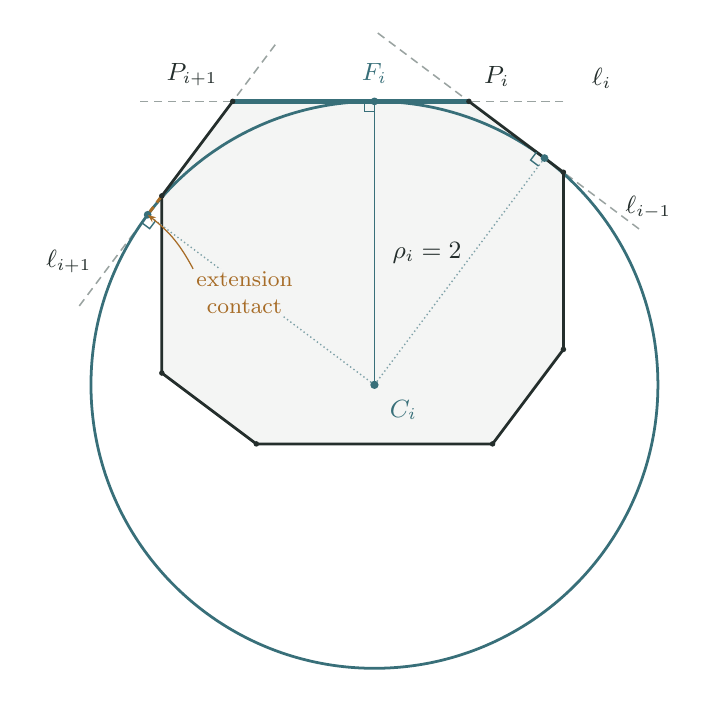
\begin{tikzpicture}[x=1.8cm,y=1.8cm,font=\small,text=ink]
\path[use as bounding box] (-3.78,-3.62) rectangle (0.82,1.02);
\coordinate (p0) at (0.000000000,0.000000000);
\coordinate (p1) at (-0.666666667,0.500000000);
\coordinate (p2) at (-2.333333333,0.500000000);
\coordinate (p3) at (-2.833333333,-0.166666667);
\coordinate (p4) at (-2.833333333,-1.416666667);
\coordinate (p5) at (-2.166666667,-1.916666667);
\coordinate (p6) at (-0.500000000,-1.916666667);
\coordinate (p7) at (0.000000000,-1.250000000);
\coordinate (c) at (-1.333333333,-1.500000000);
\coordinate (f0) at (-0.133333333,0.100000000);
\coordinate (f1) at (-1.333333333,0.500000000);
\coordinate (f2) at (-2.933333333,-0.300000000);
\fill[ink!5] (p0)--(p1)--(p2)--(p3)--(p4)--(p5)--(p6)--(p7)--cycle;
\draw[quiet,densely dashed,line width=.55pt] (0.533333333,-0.400000000)--(-1.333333333,1.000000000);
\draw[quiet,densely dashed,line width=.55pt] (0.000000000,0.500000000)--(-3.000000000,0.500000000);
\draw[quiet,densely dashed,line width=.55pt] (-2.033333333,0.900000000)--(-3.433333333,-0.966666667);
\draw[teal,line width=1pt] (c) circle[radius=2];
\draw[ink,line width=1pt] (p0)--(p1)--(p2)--(p3)--(p4)--(p5)--(p6)--(p7)--cycle;
\draw[teal,line width=1.65pt] (p1)--(p2);
\draw[gold,line width=1.05pt,densely dashed] (p3)--(f2);
\draw[teal,line width=.65pt] (c)--(f1);
\draw[teal!65,line width=.5pt,densely dotted] (c)--(f0) (c)--(f2);
\draw[teal,line width=.5pt] (-0.189333333,0.142000000)--(-0.231333333,0.086000000)--(-0.175333333,0.044000000);
\fill[teal] (-0.133333333,0.100000000) circle[radius=1.4pt];
\draw[teal,line width=.5pt] (-1.403333333,0.500000000)--(-1.403333333,0.430000000)--(-1.333333333,0.430000000);
\fill[teal] (-1.333333333,0.500000000) circle[radius=1.4pt];
\draw[teal,line width=.5pt] (-2.975333333,-0.356000000)--(-2.919333333,-0.398000000)--(-2.877333333,-0.342000000);
\fill[teal] (-2.933333333,-0.300000000) circle[radius=1.4pt];
\foreach \j in {0,...,7} \fill[ink] (p\j) circle[radius=1pt];
\fill[teal] (c) circle[radius=1.5pt];
\node[above right=2pt] at (p1) {$P_i$};
\node[above left=2pt] at (p2) {$P_{i+1}$};
\node[above=3pt,text=teal] at (f1) {$F_i$};
\node[right=3pt] at (-1.333333,-.57) {$\rho_i=2$};
\node[below right=2pt,text=teal] at (c) {$C_i$};
\node at (.27,.66) {$\ell_i$};
\node at (.60,-.25) {$\ell_{i-1}$};
\node at (-3.49,-.63) {$\ell_{i+1}$};
\node[text=gold,font=\footnotesize,align=center,fill=ink!5,inner sep=1pt] (note) at (-2.25,-.85) {extension\\contact};
\draw[gold,-{Stealth[length=3pt]},line width=.45pt] (note.north west) to[bend right=12] (f2);
\end{tikzpicture}
\end{document}
